% !TEX root = ../masterthesis.tex
\chapter{Methods}
\label{cha:methods}

\section{Optical setup}

\begin{figure}[H]
	\centering
	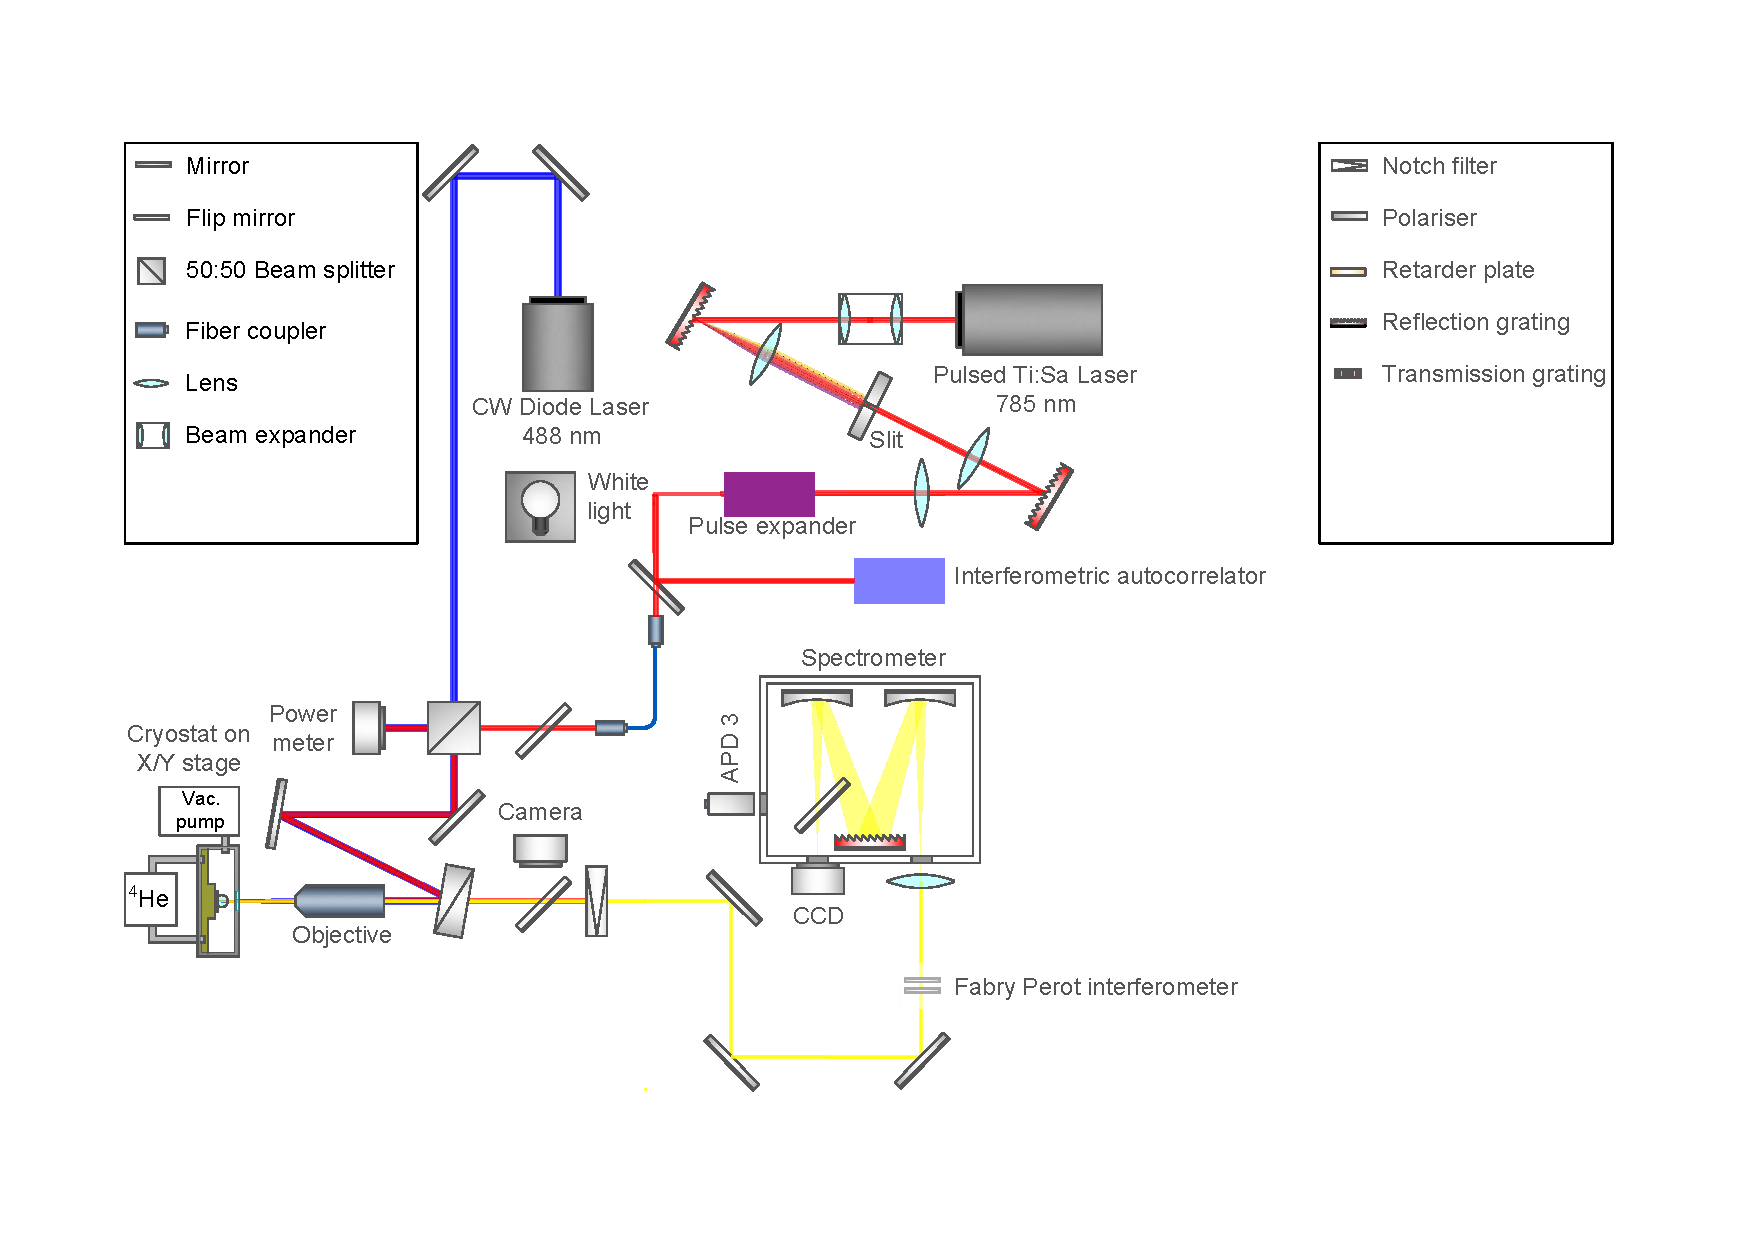
\includegraphics[width=1\linewidth]{figures/setup/Setup_flat}
	\caption[Complete experimental setup]{Complete experimental setup, which was used in order to quantify the chirp of the Ti:Sa Laser and resolve spectral emission of a quantum dot~\cite{schimpf_towards_2017}.}
	\label{fig:setupflat}
\end{figure}


The setup used for the measurements described in following chapters is sketched in figure~\ref{fig:setupflat}.
It involves a pulsed Ti:Sa laser which is sent through a pulse shaper and its chirp can be modified with the pulse expander and measured with the interferometric autocorrelator as will be discussed in chapter~\ref{cha:chirp}.
The CW diode laser is used in order to find a suitable \ac{QD} and the white light enhances the brightness of some \acp{QD} by suppressing blinking~\cite{jahn_artificial_2015}.
The spectrometer is then used to measure \ac{QD} emission either with the CCD or the APD.  

\section{Pulse shaper}

In order to resonantly excite the $\ket{XX}$ state a pulsed Ti:Sa laser with a \ac{FWHM} pulse duration of $\tau_P\approx\SI{100}{\femto \second}$ is used.
Under the assumption that the laser pulse is of Gaussian shape and that it is chirp-free (more on that in chapter~\ref{cha:chirp}), the spectral bandwidth $\Delta \nu$ can be described by~\cite{sipek_spectral_2016}
\begin{equation}
\Delta \nu \tau_P \approx 0.44.
\end{equation}
This corresponds to a spectral range of $\Delta E = h\Delta \nu = \SI{18.2}{\milli \electronvolt}$.
As can be seen in equation~\eqref{eq:e_p}, the spectral range should be smaller that $E_B/2\approx\SI{1.89}{\milli \electronvolt}$, which is not fulfilled with the laser beam alone.

The pulse shaper sketched in the upper part of figure~\ref{fig:setupflat} is used in order to tune $\Delta E$ and additionally the centre emission energy to our requirements.
The laser beam is sent through a Keplerian telescope in order to expand its beam diameter from \SI{3.4}{\milli \meter} to \SI{6}{\milli \meter}.
It gets dispersed by a diffraction grating and then focused by a lens so that the spectral components are ordered along the Fourier plane where the slit is placed.
The centre energy can be adjusted with the slit position and the spectral range with the slit width.
The setup is mirrored with an additional lens and diffraction grating, which transform the laser beam back into real space. 


\section{Micro photo-luminescence}

The following chapters will investigate the optical properties of \acp{QD}.
In order to achieve that, it is necessary to excite and collect light of only a single \ac{QD}.
This is achieved by \ac{MPL}, which involves (i) reducing the diameter of the excitation laser beam and (ii) using samples with a low \ac{QD} density~\cite{reindl_characterisation_2014}.
(i) can be improved by using an objective, where its minimal achievable spot size $d$ is described by the Abbe limit
\begin{equation}
d = \frac{\lambda}{2 \cdot NA}
\end{equation}
with $NA$ as the numerical aperture.
As the wavelength of the laser $\lambda$ is adjusted according to the optical properties of the \ac{QD}, $NA$ is the adjustable factor.
In our laboratory, objectives between $NA=0.42$ and $NA=0.85$ are used, allowing laser spot sizes in the order of the excitation wavelength.
A \ac{QD} density of approximately $1 / \lambda^2$ is therefore necessary in order to examine the emission of a single \ac{QD}.

\begin{figure}[H]
	\centering
	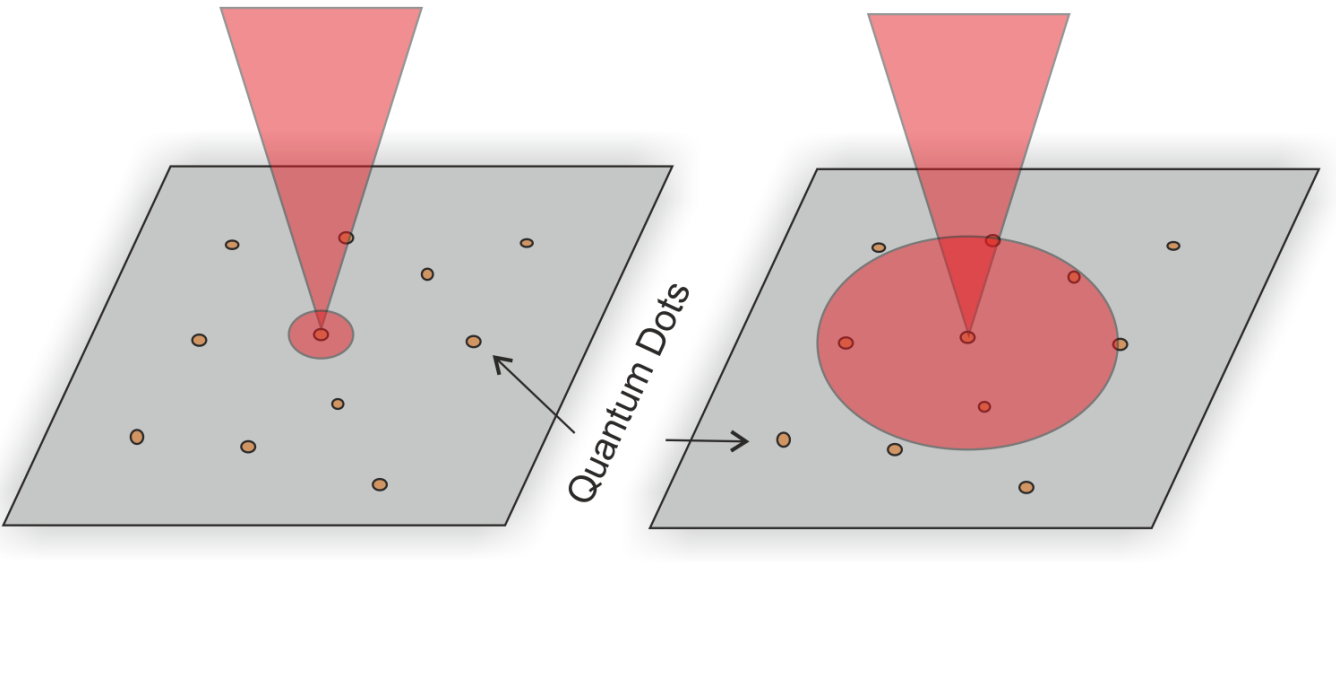
\includegraphics[width=0.7\linewidth]{figures/setup/micro-pl}
	\caption{Laser beam of different spot sizes illuminating quantum dots~\cite{reindl_characterisation_2014}.}
	\label{fig:micro-pl}
\end{figure}

The sample containing the \acp{QD} is mounted inside the cryostat, which is cooled down to \SI{4}{\kelvin}.
Without this process, the excitons would not be stable anymore, as the thermal energy would be higher than the intraband-transition energies.
The laser beam is focused on the sample by the objective and the \ac{QD} emission is then collected by the very same objective and passed through a beam splitter.
